% This is samplepaper.tex, a sample chapter demonstrating the
% LLNCS macro package for Springer Computer Science proceedings;
% Version 2.20 of 2017/10/04
% TEMPLATE: https://www.springer.com/de/it-informatik/lncs/conference-proceedings-guidelines
%
\documentclass[runningheads]{llncs}

\usepackage{graphicx}
\usepackage{todonotes}
\newcommand{\comment}[1]{}

% Used for displaying a sample figure. If possible, figure files should
% be included in EPS format.
%\usepackage{comment}
%\usepackage{lettrine} % if you want the first letter to be \letterine{b}{igger}
% If you use the hyperref package, please uncomment the following line
% to display URLs in blue roman font according to Springer's eBook style:
% \renewcommand\UrlFont{\color{blue}\rmfamily}

%\newcommand{\rom}[1]{\uppercase\expandafter{\italic\romannumeral #1\relax}}  % roman numbers with \rom{num}
%\newcommand{\ber}[1]{\lowercase\expandafter{\italic #1\relax}} % a
\newcommand{\rom}[1]{\textit{#1}}
\newcommand{\ber}[1]{\textit{#1}}

\newcommand{\reffig}[1]{Figure~\ref{#1}}
\newcommand{\reftab}[1]{Table~\ref{#1}}
\newcommand{\refsec}[1]{Section~\ref{#1}}

%\newcommand{\noteme}[1]{}
\newcommand{\noteme}[1]{\todo{#1}}
\renewcommand{\note}[1]{\todo{#1}}
\renewcommand{\bigbreak}{}

\newcommand{\quotel}{``}
\newcommand{\quoter}{''}

\newcommand{\creditfootnote}[1]{}
\renewcommand{\figurename}{Figure}

\begin{document}
%
\title{Towards Private Active Choreographies on Public Blockchain }
%
%\titlerunning{Abbreviated paper title}
% If the paper title is too long for the running head, you can set
% an abbreviated paper title here
%
\author{Jan Mensch\inst{1, 2} \and Henry Bergstroem\inst{1}}
%
\authorrunning{J. Mensch and H. Bergstroem}
% First names are abbreviated in the running head.
% If there are more than two authors, 'et al.' is used.
%

\institute{Hasso Plattner-Institut, Prof.-Dr.-Helmert-Str. 2-3, 14482 Potsdam, Germany 
\email{	bergstroem@uni-potsdam.de}
\and
University of Potsdam, Am Neuen Palais 10, 14469 Potsdam, Germany   \\
\email{jan.mensch@uni-potsdam.de}}

%
\maketitle              % typeset the header of the contribution
%
\begin{abstract}
    Integrating business processes has been found to have a positive impact on operational and business performance \cite{flynn2010impact,narayanan2011antecedents}. However if business partners have little trust in each other, integrating processes is challenging \cite{panayides2009impact}. In this paper an approach towards a realization of Active Choreographies (ACs) is presented, that is in no need of trust and can enforce a business process, while still implementing strong visibility constraints that would usually be required in real-world applications. These constraints keep the business logic, the identity of a message originator and the content of their communication secret. This is done while still being able to record an encrypted audit trail, where messages are only readable by parties that are allowed to read them. There also exists an implementation of a prototype, which showcases the proposed scheme.
\end{abstract}

\section{Introduction} \label{sec:intro}

Integrating business processes has been found to have a positive impact on operational and business performance \cite{flynn2010impact,narayanan2011antecedents}. However such progress is hindered, because there is a lack of trust between the collaborating businesses \cite{panayides2009impact}. The proposed solution is in no need of trust between participants, in no trust of any central authority and keeps the business done secret, which might improve collaboration between businesses. As shown by Weber et al., there are ways to extend the use cases of business process execution and auditing to an untrusted environment, thus making it possible for entities to collaborate with each other that would usually not be willing to do so \cite{weber2016untrusted}. This execution of untrusted business processes is made possible by using an blockchain-based implementation of Active Choreographies, briefly discussed in \refsec{subsec:blockchainbased}.

The goal of this paper is to explore the notions of privacy and visibility with regards to untrusted execution of choreographies on the blockchain\footnote{A blockchain can be thought of as a decentralized state transition system, where the nodes in the blockchain networkn agree on a new state by appending it to the blockchain. By making the addition of a new state computationally hard, a blockchain can ensure that it is very difficult to change already commited steas \cite{buterin2014next}. } and to introduce a scheme which aims to keep untrusted business process execution private, while still being enforceable. The structure of the paper is as follows: Background (\refsec{sec:background}), which give a short overview of the work considered when creating the solution. Approach (\refsec{sec:approach}), which describes the proposed solution. A brief explanation of the architecture of the proposed solution. Implementation (\refsec{sec:eval}) and the discussion (\refsec{sec:discussion}). A summary over limitations, alternative implementation and future work. The paper closes with the chapter Conclusion (\refsec{sec:conclusion}), which is a summary of the findings of this paper.

\section{Background} \label{sec:background}

\subsection{Blockchain-Based Choreographies} \label{subsec:blockchainbased}

The following section provides a short introduction to blockchain-based choreographies. 

\textbf{Active Mediators.} Weber et al. explain how a business process can be enforced in an environment where the participants do not trust each other \cite{weber2016untrusted}. This is done by using a smart contract\footnote{A program which is being executed on a blockchain.}, acting as an active mediator between participants. The term active mediator implies that the component is able to accept or reject messages and makes sure that the business process is executed as specified. With the help of this and other components Weber et al. are able to (I) execute collaborative processes over a network of untrusted nodes, (II) enforce that only conforming messages can trigger state changes. The implementation also for (III) payments and escrows to be coded in the business process and (IV) an immutable audit trail, that keeps track of all transactions. Furthermore, none of the participants in the business process has to control the collaboration, which is what differentiates a choreography from an orchestration. The approach introduced in by Weber et al. is different from ours in the sense that in their implementation the business process is included in the smart contract, which makes it public. It displays which participants are collaborating with each other, how they are doing it and what messages are exchanged. The aim is to provide privacy and try to hide the logic of the business process, who the originator of a message is  and what messages are exchanged, while still providing that (I), (II) and (IV) hold.


\textbf{Active Choreographies.} Ladleif builds on the work of Weber et al. and creates an extension of the Business Process Model and Notation (BPMN) 2.0 choreography diagrams in combination with Ethereum. The introduced addition to the BPMN standard is capable of modeling events, scripts and data, which are vital to the modeling of smart contract driven choreographies. This extension is called Active Choreographies. Like   Weber et al., Ladleif uses smart contracts as a central link between the collaborating parties. Messages are not exchanged directly between the entities, but through the smart contract. This scheme allows for business process execution without the need of trust between the participating businesses \cite{ladleif}. 


The work presented in this paper is a realization towards Active Choreographies, which are in no need of trust and can enforce a specified business logic. The addition of this work to the work of Weber et al. and Ladleif is the provision of strong visibility constraints. 

The work presented here is thus work towards private Active Choreographies on public blockchain infrastructure. 




\subsection{Visibility Levels} \label{subsec:levels}

While the issue of privacy was mentioned by Weber et al. and Ladleif, they did not take any measures to actually implement them. However, Ladleif did introduce different levels of visibility in the context of modeling business contracts with ACs \cite{ladleif}. The levels are as follows:



\begin{itemize}
    \item \ber{Model Level}: The logic of the business process. If you would model a business process using BPMN, the BPMN model would be the model layer. If you would implement it using a programming language, the source code would be the model layer.
    \item \ber{Communication Level}: The knowledge of which messages were exchanged, who exchanged them and which entities are part of the business process. Ladleif also includes the time at which messages were sent. For the scope of this publication,
    the time of an exchanged message is excluded from the communication level.
    \item \ber{Content Level}: The content of the exchanged messages.
\end{itemize}

It is referred to these levels in \refsec{subsec:assumptions} when the assumptions that the approach is based on are discussed.




\subsection{Privacy Enhancing Technologies} \label{subsec:technologies}

The proposed implementation aims to provide privacy for all three layers. Multiple other technologies that are worth mentioning and could be a viable alternative to the presented approach were considered. Some of these technologies are discussed again in \refsec{subsec:alternative} in the context of using them for alternative implementations.


One of them is \textit{obfuscation}. This is a technology that \quotel aims to make a computer program `unintelligible'\ while preserving its functionality\quoter  \cite{garg2016candidate}. Since it was shown in that there is a set of functions that are impossible to obfuscate, the idea of indistinguishability obfuscation  was introduced \cite{barak2001possibility,barak2012possibility}. This is a weaker constraint, guaranteeing that it is impossible to distinguish two equivalent programs of a similar size that have been obfuscated. These ideas seem to be very powerful, but come with a big drawback: Being so computationally expensive that they are practically unusable \cite{banescu2015idea}.

\textit{Homomorphic encryption} might be used to do calculations on encrypted values. Similar to obfusaction, homomorphic encryption suffers from heavy computational overhead \cite{gentry2010computing}.


A further technology considered is \textit{secure multi-party computation (SMPC)} \cite{orlandi2011multiparty}. With SMPC, there are multiple parties involved in computing the output of a function. These parties do not have to trust each other. Therefore, they need a protocol that makes sure that the output is correct and that cheating participants will not be able to learn anything about the input of the honest parties. 


A technology already in use in blockchain applications are \textit{zero-knowledge Succinct Non-interactive ARguments of Knowledge (zk-SNARKs)}. An application using them is Zerocoin, which aims to provide  \quotel fully anonymous currency transactions\quoter  \cite{miers2013zerocoin}. zk-SNARKS provide the possibility to have an untrusted prover verify a statement (or secret) made by a different party, without that party having to reveal their secret \cite{ben2013snarks}. It furthermore does so in a non-interactive manner. 

Today there are already multiple projects that focus on business process execution (e.g. Hyperledger Grid \cite{hyperledger}). Some of these implementations provide mechanisms aiming to create trust between participants. One of them is \textit{Parity Ethereum}. With Parity, users are able to hide private contracts in public contracts and to exchange private messages \cite{parity}.

\comment{
However for private contract execution Parity is relying on validators,  \quotel  account[s] that can allow a private contract’s state [to] change\quoter  \cite{parity}. In our understanding this makes Parity insufficient for untrusted business execution, since, like private blockchains, it requires trust in one or multiple nodes. 
}




\section{Approach} \label{sec:approach}

\subsection{Assumptions and Scenario} \label{subsec:assumptions}

Before the introduction of the scheme, the underlying assumptions and opinions are introduced. Each assumption is marked with a letter for later reference. Please note that the authors are aware that in reality not all of the assumptions will hold. The assumptions are listed to describe a setting where private active choreographies on public blockchain are possible.

\begin{itemize}
    \item \textit{Assumption about the visibility levels}: It is assumed that the participating entities want to keep all levels discussed in \refsec{subsec:technologies} secret. This includes their business process, with whom they are communicating and what is being communicated. 
    \item \textit{Assumptions about the blockchain infrastructure}: It is assumed that every operation done on the blockchain is public. This includes all data that is being processed on-chain. It is further assumed that a public blockchain is superior to a private one in terms of trust, since it does not require trust in the organisation that runs the network. In addition to that it is the authors oppinion, that a network that employs \quotel  policing nodes\quoter \footnote{Nodes that have the special role of enforcing rules.} is inferior to a network without such nodes, since such a network requires \quotel trust in the authorities\quoter. Another assoumption about the underlying network is, that the communication between nodes is done via a message-based system where the metadata of a message does not contain the address of the message sender.
    \item \textit{Assumptions about the participating entities}: There are several parties which want to collaborate. These parties have neither trust in each other nor  trust in any third party. Since the parties distrust each other they also  only want to share messages with the entities that have to see them and keep them secret from the others.
    It is furthermore assumed, that each party  is  \quotel  honest-but-curious\quoter  \footnote{Definition honest-but-curious:  \quotel The honest-but-curious (HBC) adversary is a legitimate participant in a communication protocol who will not deviate from the defined protocol but will attempt to learn all possible information from legitimately received messages.\quoter  \cite{paverd2014modelling}}.
\end{itemize}


\comment{
\bigbreak
\textbf{Assumptions about the participating entities}: There are several parties which want to collaborate (\ber{a}). These parties have neither trust in each other (\ber{b}) nor  trust in any third party (\ber{c}). They furthermore want to keep their business processes secret (\ber{d}),  hide with whom they are collaborating (\ber{e}) and  hide what is being communicated during the collaboration (\ber{f}). Since the parties distrust each other they also  only want to share messages with the entities that have to see them and keep them secret from the others (\ber{g}). Each party  is  \quotel  honest-but-curious\quoter  \footnote{Definition honest-but-curious:  \quotel The honest-but-curious (HBC) adversary is a legitimate participant in a communication protocol who will not deviate from the defined protocol but will attempt to learn all possible information from legitimately received messages.\quoter  \cite{paverd2014modelling}}(\ber{h}). These assumptions justify the aim to keep all levels mentioned in \refsec{subsec:levels} private. To be more specific, \ber{d} requires a private \ber{Model Level}, \ber{e} a private \ber{Communication Level} and \ber{f} a private  \ber{Content Level}.

\bigbreak
\textbf{Further assumptions:}
All data that is processed on the blockchain is considered public (\ber{i}). It is possible to convert a business process into a program or state-machine in order for parties to determine the validity of a state change (\ber{j}). The process of converting a business process into a program or state-machine is out of the scope of this paper. In our opinion a public blockchain is superior to a private one in terms of trust, since it does not require trust in the organisation that runs the network (\ber{k}). We furthermore believe that a network that employs \quotel  policing nodes\quoter \footnote{Nodes that have the special role of enforcing rules.} is inferior to a network without such nodes, since such a network requires \quotel trust in the authorities\quoter (\ber{l}). Communication between nodes is done on a message based system where the metadata of a message does not contain the address of the message sender (\ber{m}).
}

\begin{center}
\begin{figure}
    \centering
    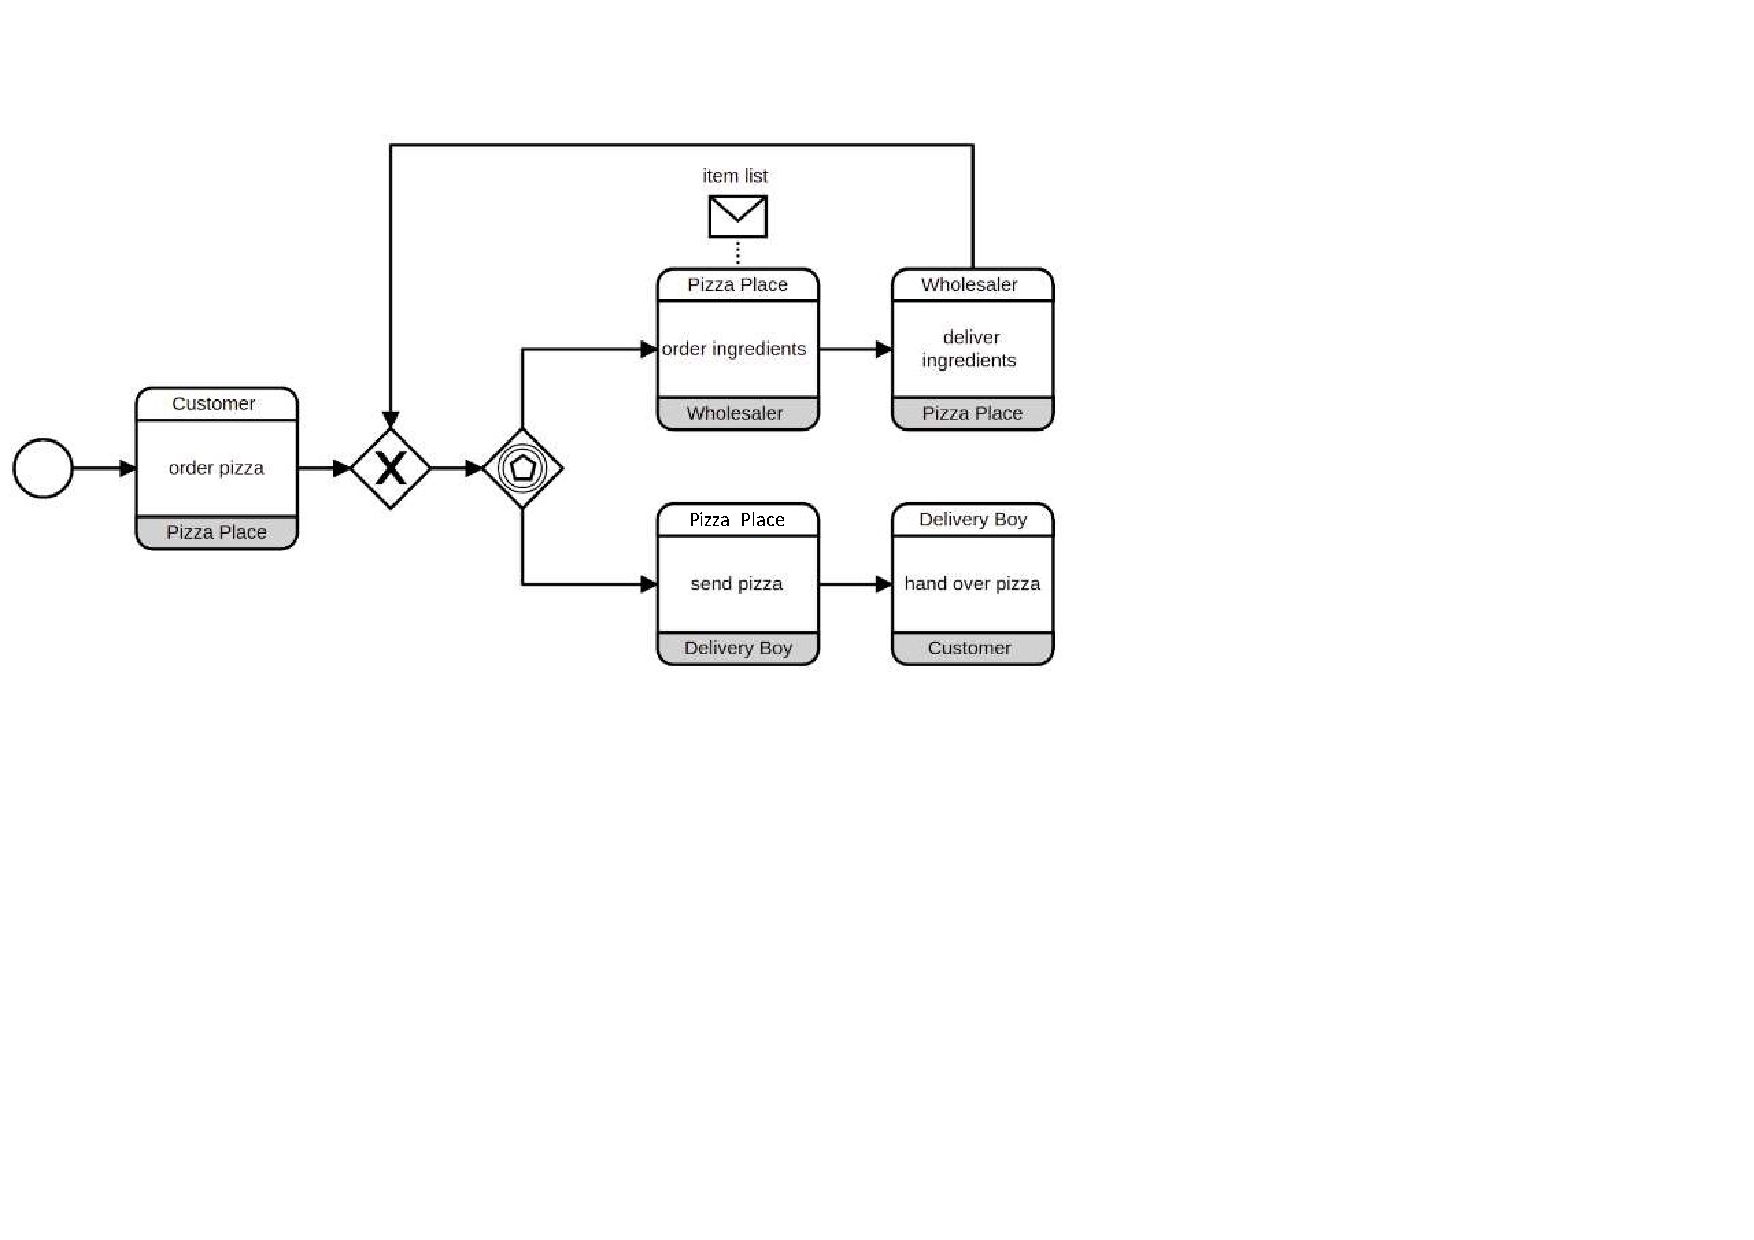
\includegraphics[trim=0cm 9.5cm 11.5cm 2.4cm,clip=true,scale=0.65]{newbpmn.pdf}
    \caption{Choreography diagram of a pizza ordering process} 
    \label{fig:simple_bpmn}
\end{figure}
\end{center}

%\noteme{process send pizza is supposed to be between pizza place and delivery boy.}

Throughout this paper arguments are presented in a more concrete fashion, by applying them to the example shown in \reffig{fig:simple_bpmn}. Here the parties are collaborating without trust (\textit{Assumption about the participating entities}). They also have an urge to keep as much as possible about their collaboration secret (Assumptions about the visibility levels). An example of the \textit{assumption about the participating entities} would be, that the \textit{Delivery Boy} (\ber{D}) should not know anything about the collaboration between the \textit{Customer} (\ber{C}) and the \textit{Pizza Place} (\ber{P}), even though \ber{D} is part of the overall business process. 



\subsection{Proposed Scheme} \label{subsec:scheme}


This chapter is discussing the proposed schema. This is done by introducing mechanisms which each solve one or more of teh assumptions of \refsec{subsec:assumptions}.


\textbf{Circles.} In order to keep the \textit{content level} secret, the notation of circles is introduced. Circles are visibility constraints for a group of entities. A message exchanged within a circle can only be read by other participants of a circle. This is achieved by this using symmetric keys which are exchanged between the members of a circle before the execution of the process. This can be done by using well established protocols like the session key exchange in openPGP \cite{openpgp}. Which parties are within which circle should be established by the parties themselves and is therefore out of scope of this paper. \reffig{fig:circles} shows an example of possible circles of the process defined in  \reffig{fig:simple_bpmn}. Each circle has its own associated symmetric key and each message is encrypted with the respective key. This way \ber{C} cannot read the communication between the \ber{Wholesaler} (\ber{W}) and \ber{P}, because this communication is encrypted with ${sym}_2$ and \ber{C} is only in possession of ${sym}_1$. Also the message can still be included in the audit trail, since only members that are in possession of ${sym}_2$ can read it.\creditfootnote{Credit: key-icons in \reffig{fig:circles} made by Yannick (http://yanlu.de) from www.flaticon.com}


\begin{center}
\begin{figure}
    \centering
    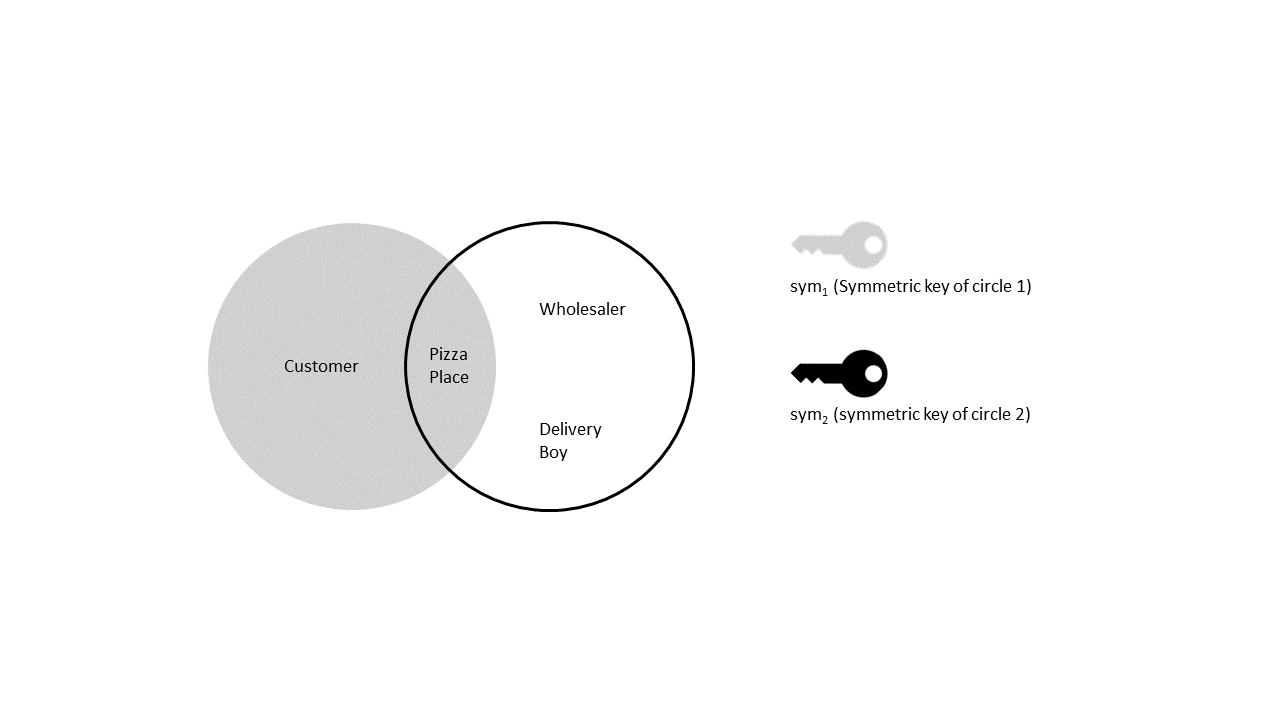
\includegraphics[trim=0cm 0cm 0cm 0cm,clip=true,scale=0.25]{circles.png}
    \caption{Circles of the process described in \reffig{fig:circles}. The circles indicate who is communicating with whom and who should see the content of the exchanged communication.} 
    \label{fig:circles}
\end{figure}
\end{center}



\bigbreak
\textbf{Protecting the Model Layer.} Since all communication and all code executed on the blockchain is considered to be public  (assumption \ber{i}), the logic and execution is done off-chain. This is in order to keep the \ber{Model Layer} secret (assumption \ber{d}). The representation of the business process is shared amongst all entities. This could be a graph or executable code (assumption \ber{j}). This representation should vary in detail, hiding the details of the process that are out of the own circle. How this representation looks like exactly and how it is shared is out of scope of this paper.


\bigbreak
\textbf{Consensus Mechanism.} Since the logic of the business process is stored off-chain, a smart contract (sc) has no way of knowing if a proposed state change is valid or not. This is why a simple consensus mechanism for the nodes and a sc that is able to reject messages that did not result out of this consensus mechanism were created. If both of these things are given a smart contract is able to enforce a business process without being aware of its logic. 

In the oppinion of the authors, a business process can be viewed as a state-machine. In it, states are actions that are taken by the entities (e.g. \quotel send pizza\quoter ) and state changes are triggered by messages (e.g. \quotel W now hands over 1kg of flour, ordered by P\quoter  changes the state from \quotel order ingredients\quoter \  to \quotel deliver ingredients\quoter ). If the state machine is automated on each client, invalid messages can be rejected and the business process enforced (the limitations of this approach are discussed briefly in \refsec{sec:discussion}).

\begin{center}
\begin{figure}
    \centering
    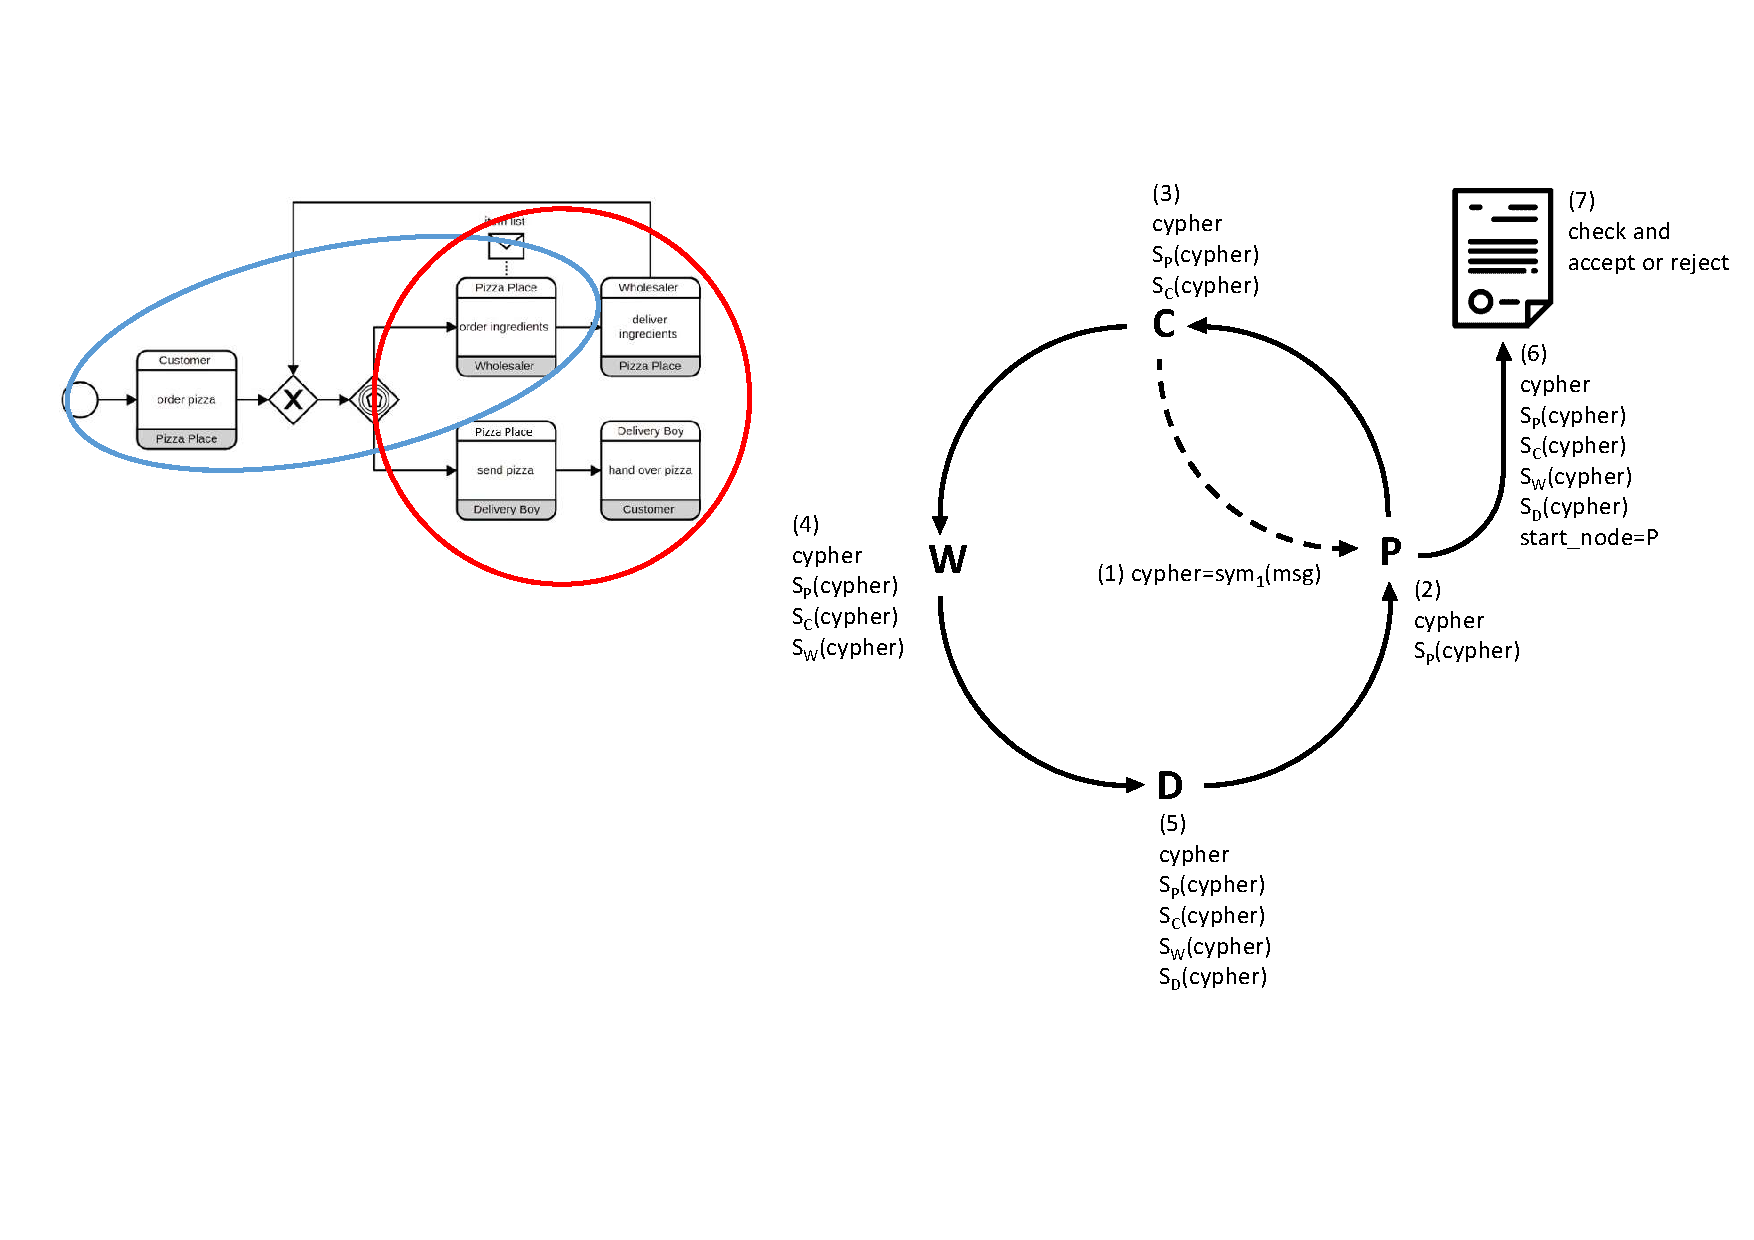
\includegraphics[trim=13cm 4cm 0cm 3cm,clip=true,scale=0.5]{schema.pdf}
    \caption{The proposed scheme. 1: initial sending of cypher. 2-5: other nodes give consent. 6: cypher and signatures are send to smart contract. 7: validation} 
    \label{fig:scheme}
\end{figure}
\end{center}


\reffig{fig:scheme} shows such a mechanism\creditfootnote{Credit: contract-icon in the \reffig{fig:scheme} made by Freepik (http://www.freepik.com) from www.flaticon.com}. In it all nodes are placed in a ring\footnote{Not to be confused with a ring-signature \cite{rivest2001leak}.}. In this example communication is done counterclockwise. The order in which communication is done is fixed. Just the start and endpoint vary. As already discussed, all nodes are in possession of the symmetric keys of their associated circles. In addition to that, they also own an asynchronous key-pair of which their public key is published on the smart contract.

\reffig{fig:scheme} displays how the \ber{Customer (C)} would like to propose a state change (e.g. from the \quotel start-state\quoter  to \quotel order pizza\quoter ). For that, \ber{C} creates the message \ber{msg} (e.g. \quotel C: order pizza margarita for 8 EUR.\quoter ). This message is encrypted using the symmetric key ${sym}_1$ of his circle. The encrypted message is denoted as \ber{cypher}. As a first step, \ber{C} is then sending \ber{cypher} to a random node, e.g. \ber{P} (the necessity of this step is explained in the next paragraph). Since \ber{P} happens to be in the same circle as \ber{C}, he can read \ber{cypher} by decrypting it with ${sym}_1$. 



\ber{P} can now signal his consent by applying a hash function to \ber{cypher} and then encrypting this hashed value with his private key. The combination of these functions for the signing process is denoted as $S_X$. $X$ is the name of respective node. A node that is not in the circle does not receive any new information since it is not able to read the message. It is also unable to know who the originator of the message is, since the originator sends it to a random node to start the procedure. If this was not the case and \ber{C} would send \ber{cypher} the next node in line (\ber{D}), \ber{D} would know that \ber{C} is the message sender, since the order of nodes is known to all entities. This is done in accordance with the assumptions about the participating entities. 


If all nodes \quotel agreed\quoter \footnote{\quotel Agreed\quoter, since nodes outside the circle cannot read the message and simply pass it on.} to \ber{cypher}, \ber{cypher} and the signatures will reach \ber{P} again. Since \ber{P} has already seen \ber{cypher} he will send it to the smart contract for validation, together with all signatures and the information that he was the first node to add a signature (\ber{start\_node=P}). If the validation passes, the nodes will know that they reached a new state in their business process, but only \ber{C} and \ber{P} will know what state this is.



\subsection{Validation} \label{subsec:furtherinfo}

The smart contract receives \ber{cypher}, a list of signatures and the information that \ber{P} started the signing process. The sc can now decrypt each signature using the public key of each of node in the circle. If all encrypted signatures match the hash of \ber{cypher} the state change is valid. \ber{cypher} is then included in the audit trail and all clients know that a new state was reached, but only \ber{C} and \ber{P} will know which state this is, since only they are in possession of ${sym}_1$. This way an audit trail is kept in which messages can only be read by entities that are supposed to read them.


\section{Implementation} \label{sec:eval}


In order to evaluate the approach, a simplified version of the scheme discussed in \refsec{fig:scheme} was build. The clients were implemented using Python 3.6 and the smart contract was implement using Solidity running on a local Ethereum Blockchain on Ganache. The implementation is able to simulate a ring with three nodes. If all nodes confirm the encrypted message by signing it, the encrypted message and the signatures are sent to the smart contract for validation. Out of the three clients, two are in the same circle. This is to showcase the visibility constraints of circles. 

So far, the automatic accept or reject mechanism that is necessary to enforce a business process was not implemented. With the current prototype, a user has to accept or reject the proposed state change manually. 

Topic of future work is also the algorithm deciding to which random node an encrypted message should be sent at the first step of the scheme. With the current implementation the client just sends it to the next node in line. The topic of choosing a random node was avoided, because in our opinion this should be done not by the message originator, but by the entire group. This is to avoid the danger that a node might choose a different node not at random but with the intention to somehow cheat on the system.


\comment{
done: 
simple implementation 
simulating a simple ring with 3 clients 
2 clients are within the same circle 
smart contract has public and is able to verify messages send from the ring

Not done: 
randomization. A client will not send the message of to a new node, rather just to the next one in line

Automatic accept/reject of messages send from node to node. User has to do that at current time.

architecture: 
Clients implemented in Python 3.6

smart contract implemented using Solidity

Application was tested using the local Ethereum application Ganache

}


\section{Discussion} \label{sec:discussion}

\subsection{Limitations of the Proposed Scheme}

There are a number of shortcomings in the approach that was introduced in \refsec{subsec:scheme}. In this chapter a few of the will be discussed.



\bigbreak
\textbf{Collusion of all entities within a circle.} The goal of our approach was to enforce a business process, while keeping the \ber{Model Layer}, the \ber{Communication Layer} and the \ber{Content Layer} secret. This is achieved by automatically rejecting illegal state changes. If an entity encounters a message proposing an impossible state change it should reject it (at least if it is able to read that message). A possible misuse of this system is that all entities within a circle collaborate and pass invalid state changes. It is debatable though if this behaviour should be prevented. Messages passed within a circle should be only relevant for the parties within that circle. If the deviation from the defined business process is agreed upon by all parties within the circle, this would be equivalent to renegotiating the terms of the collaboration. For example, \ber{C} might send the message \quotel send pizza margarita for 6 EUR\quoter , even thought the price might have been defined as 8 EUR in the business process. If \ber{P} now accepts it, they just renegotiated their terms. The way the business process is enforced is therefore rather soft. 


\bigbreak
\textbf{Knowledge of progress within the consensus mechanism.} During the consensus mechanism every entity is adding their signature to the message which is passed around. Because the sc has to know all public keys in order to verify messages, the number of participants is known to all entities. Every node who receives this message will therefore be aware of how important their consent it (premise \ber{h}). This knowledge might be abused and should be avoided.


\bigbreak
\textbf{Blocking progress.} Any node can decide to not sign any more messages and block the progress of the business process. It is assumed that this issue will not occur very often, because the nodes that are participating in the business process should have an interest in the successful execution of that progress (\textit{assumption about the participating entities}).


\bigbreak
\textbf{Powerful nodes.} Depending on the business process and the participating parties, it might happen that there is an party that accumulates a lot of knowledge. In our case this is \ber{P}, who can see all messages exchanged, because he is a member in both circles. This may or may not be seen as a problem by the other participants. This issue should be taken into account when designing the visibility constraints of the business process. 


\bigbreak
\textbf{Spam.} If assumption \ber{m} holds and the nodes indeed do not know who the originator of a message is, this opens the door for spam messages. An outsider could send a message, encrypted with an unknown key to a member of the ring. That member would pass the message along, assuming that he can not read it because he is not part of the same circle as the originator of the message. So would all other nodes in the ring and the message would be verified by the sc and stored on the blockchain. Depending on which blockchain is used, storing data on it might be expensive. An outsider might therefore be able to increase the price of the business process execution. This should be avoided! A possible solution to this might be to have all nodes create a second key-pair and to only exchange those public keys within the ring. These public keys might then be used to create a ring signature \cite{rivest2001leak}, which would prove that the originator of a message is indeed part of the ring. The \quotel original\quoter  public keys could not be used for this task, since they are encoded in the sc and are therefore public knowledge (\textit{assumption about the blockchain infrastructure}).



\subsection{Alternative Approaches} \label{subsec:alternative}

Some of the technologies mentioned in \refsec{subsec:technologies} might be used to provide privacy. For example, zk-SNARKs might be used to prove that a state change is legal. If that would be possible, it might be possible to design a protocol in which the communication overhead between the nodes could be drastically reduced. 

%\todo{write about ofuscation?}

It was only possible to read about a few of the many block\-chain-im\-ple\-men\-ta\-tions that take on the issue of privacy. The one implementation that stood out was Parity Ethereum, which is why it is mentioned in \refsec{subsec:technologies}. As already discussed, users are able to create private contracts and to exchange private messages. However one difference between this approach and Parity is that Parity needs specialized nodes in order to execute private contracts. These nodes are called validators, which are \quotel account[s] that can allow a private contracts state change\quoter  \cite{parity}. In the authors opinion this trust in specialized nodes makes Parity unfit for untrusted business process execution (\textit{assumption about the blockchain infrastructure}).

\comment{
We would also like to mention Parity Ethereum. With Parity, users are able to hide private contracts in public contracts  and to exchange private messages. However for private contract execution Parity is relying on validators, \quotel account[s] that can allow a private contract's state change\quoter  \cite{parity}. In our understanding this makes Parity unfit for for untrusted business process execution, since, like private blockchains, it requires trust in one or multiple nodes.

\todo{Parity comparison}
}
\section{Conclusion} \label{sec:conclusion}

\comment{
\begin{itemize}
    \item How could mentioned in \refsec{subsec:technologies} improve \refsec{sec:eval}?
    \item How did it work out in the end? 
\end{itemize}}

In this paper it was shown, that it is possible to hide the logic of the business process, the communication and the content of the messages. This was achieved on public blockchain infrastructure to avoid the trust issues that are, in the opinion of the authors, inherent to private blockchains. It was furthermore shown that a business process can be enforced without the smart contract being aware of its logic. Since this work is proprietary, there are multiple limitations to it. For some of these limitations solutions were proposed. The authors would like to express their hope, that this paper might be a first step towards private active choreographies on public blockchain.





\bibliographystyle{IEEEtran} % BibTeX users should specify bibliography style 'splncs04'.
\bibliography{refs} % Entries are in the "refs.bib" file


\end{document}

